Una vez corroborado que el error ya no ocurrió nuevamente, se procedió a ingresar la señal del lazo de corriente para controlar el variador de velocidad.

Para la comunicación del Arduino con el variador de velocidad se decidió utilizar un lazo de corriente de 0-20mA, este tiene ventajas sobre el lazo de tensión ya que el utilizado es más estable en largas distancias y más inmune a los ruidos eléctricos e interferencias electromagnéticas respecto al lazo de tensión. Normalmente, se utilizan lazos de corriente de 4-20mA para poder observar si hubiera fallas en el circuito, pero este modelo de variador, tiene el piso del lazo de corriente en 0mA. Cabe mencionar, que el variador podía ser controlado por cualquiera de los dos métodos de lazos.

A continuación se observará la placa interna del variador con sus respectivas borneras por donde ingresará la señal de corriente del lazo de control y el jummper que se tuvo en cuenta para que sea de corriente y no de tensión.


IMAGEEEN

La señal para controlar el variador de velocidad fue generada por una señal PWM estipulada a través de la librería TIMEROne. La instrucción Timer1.inizialize(period)
 de Arduino inicializa el timer con el valor de period, este valor es el tiempo en el que se dispara el temporizador y en el caso de este proyecto es de 40 microsegundos.
El otro comando que se utilizó fue Timer1.pwm(pin, duty) que establece el número de pin, en este caso pin 9 y “duty” es un valor entre 0 y 1023 establecido por la programación. 
Esta señal de salida, fue necesario transformarla al lazo de corriente utilizado para establecer la señal al variador de velocidad. Esto se realizó a través de una placa adaptadora con un filtro generada por nosotros.

PROTEUS PLACA


\subsection{Captura de datos por puerto serie}
\begin{tcolorbox}[colback=blue!5!white,colframe=blue!75!black,title=Processing]
    Es un lenguaje de programación basado en Java, aunque hace uso de una sintaxis simplificada y de un modelo de programación de gráficos.
    \end{tcolorbox}
Para capturar los datos, primeramente se utilizó Matlab, como se necesitó visualizar los valores en tiempo real y luego guardar la tabla con vectores, este programa producía errores en la capturación de datos.
Para solucionar el inconveniente anteriormente nombrado, se utilizó un código generado en Processing. Con este código, se capturó los valores, se observaba el valor numérico estimado de la velocidad y se lograba ingresar el valor del escalón requerido para tomar la planta. (Figura \ref{fig:Proce})

\begin{center}
    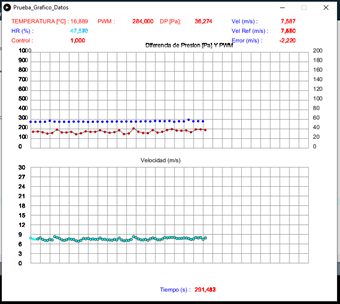
\includegraphics[scale=0.7]{serial_proc.png}
    \captionof{figure}{Pantalla Processing}
    \label{fig:Proce}    
\end{center}

\subsection{Estimación de la planta}
    \subsubsection{Diagrama de trabajo}

Para realizar la estimación de la planta se genera un diagrama de bloques del procedimiento que se siguió de forma resumida.

\begin{figure}[htb]
	\centering
	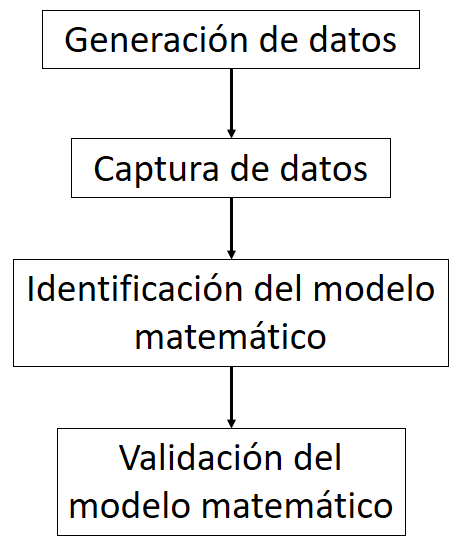
\includegraphics[scale=0.4]{planta_d.png}
	\captionof{figure}{Diagrama de bloques del procedimiento de modelado de la planta}
	\label{fig:planta_d}
\end{figure}

 \textbf{Generación de datos:}  se hizo diversas pruebas para obtener la mayor cantidad de información en la respuesta.

 \textbf{Captura de datos:} A través del puerto serie y con Processing se realiza el almacenamiento de los datos de respuesta del sistema ante el estímulo de las señales de excitación. Posteriormente, el análisis de los datos y la generación de las gráficas correspondientes es realizado por medio de rutinas de código implementadas en Matlab.

 \textbf{Identificación del modelo matemático:} Se utilizaron varios métodos numéricos para la estimación.

 \textbf{Validación del modelo matemático:} una vez obtenida la mejor estimación, se efectuó una validación adicional a partir de la comparación de datos experimentales con los teóricos generados por escalones.






    \subsection{Método de estimación}
\hl{ver si ponemos este diagrama}
    \begin{center}
        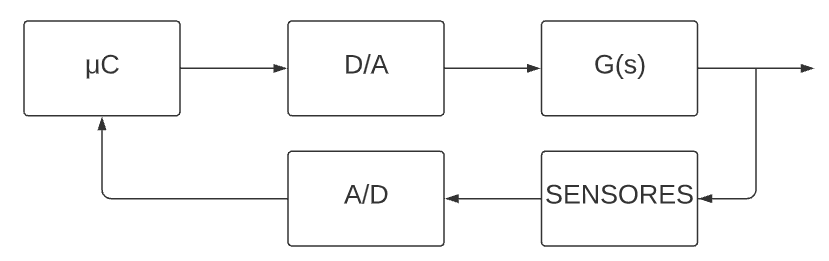
\includegraphics[scale=0.35]{bloques.png}
        \captionof{figure}{Diagrama en bloques}
        \label{fig:bloques}    
    \end{center}
       

    Una vez que se determinó valores de ventana de filtro, velocidad de conmutación de PWM, tiempos de aceleración y desaceleración, etc. Se utilizó el modo de ingreso de señal por lazo de corriente en el variador de velocidad. Para realizar la estimación de la planta se obtuvieron y guardaron tablas de datos con Processing, generando diversas señales con distintos escalones de entrada. 
    PONER PRUEBAS VALOR DEL ESCALON, VALOR DE FRECUENCIA.
    
    El archivo generado fue un “.csv” para el cual luego fue necesario utilizar un código de Matlab para obtener cada vector según los datos que poseía cada uno. Con estos datos, se realizó la estimación de la planta por los métodos de … y de……. . concluyendo que el método JSadas de cuarto orden era suficiente.
    
    1.GRAFICO Y ECUACION DE JASKAC.
    2.Grafico de los graficos con los valores marcados que se tomaron
    
    Para corroborar la elección de la planta se genreó un archivo en simulink generando como entrada los esclaones que se colocaron en el sistema.
    
    IMAGEN SIMULINK
    
    FUNCION DE TRANSFERENCIA

    
    \subsection{PID inicial}